\chapter[Le stage \ensg]{Le stage}

\section{Généralités}

Dans la suite de ce rapport je vais me consacrer sur les deux missions principales que j’ai réalisées à Galigeo. La première est l’estimation d’un flux piéton à une adresse donné. (2.2) Ce n’est pas une mission réalisée pour un client en particulier, c’est une fonctionnalité qui a été ajouté dans la dernière version des logiciels SaS de Galigeo et est donc accessible pour tous les utilisateurs du service.

\paragraph*{}

La deuxième mission est une demande spécifique d’un client de Galigeo. J’ai eu accès à des données confidentiels à l’entreprise. Toutes les illustrations, schémas ou fragments de données, pour cette partie, seront donc fictifs

\paragraph*{}

Enfin, je terminerai rapidement sur deux autres missions clients, plus secondaires pour lesquels je rentrerai moins dans le détail.


\section{Prédiction de flux piéton}

\subsection{Mise en contexte}

Le flux piéton est une très bonne variable pour estimer le flux de consommateur potentiel qui passe chaque jour devant une enseigne commerciale. Il est donc essentiel pour une entreprise qui fournit des services de géomarketing, de pouvoir estimer au mieux cette variable.

\paragraph*{}

Jusqu’aujourd’hui, Galigeo s’appuyait sur des estimations calculées par une autre entreprise ce qui l’empêchait de corriger les biais et erreurs possibles. Elle n’avait pas la main sur les algorithmes d’estimations.

\paragraph*{}

Ma mission a donc été de réaliser cet algorithme d’estimation du flux moyen de piéton sur une année autour d’une adresse donnée et ce pour l'ensemble du territoire nationale.

\paragraph{}

Il a fallu néanmoins prendre en compte les contraintes techniques de l’entreprise, les biais qui pouvait être présent dans la donnée utilisée et l’efficacité de l’algorithme. Si les temps de calculs sont trop longs, l’expérience utilisateur risque d’être impactée mais il faut garder un modèle puissant afin de minimiser les erreurs de prédiction.

\subsection{La donnée}

Pour estimer ce flux piéton, nous allons nous appuyer sur des mesures quotidiennes que Galigeo achète à un fournisseur. En effet, Galigeo reçoit quotidiennement des positions de cellulaires sur l'ensemble du territoire métropolitain. Elle en reçoit environ 70M par mois, chacune correspond à un évènement de visite. Cette donnée est collectée via des applications mobiles qui sont autorisées à transmettre au fournisseur de Galigéo la position du smartphone. Les positions sont anonymes mais possède un identifiant de smartphone ce qui permet d'avoir aussi des informations de déplacements. La donnée brute est structurée comme ci-dessous :

\begin{table}[H]
    \centering
    \begin{tabular}{|l|l|}
    \hline
    \textbf{Attribut} & \textbf{Description}              \\ \hline
    idEvent           & Id de l'évènement                 \\ \hline
    uuid              & Id du smartphone                  \\ \hline
    latitude          & Latitude de l'évènement           \\ \hline
    longitude         & Longitude de l'évènement          \\ \hline
    accuracy          & Précision de la localisation      \\ \hline
    arrival           & Date d'arrivée à la localisation  \\ \hline
    departure         & Date de départ de la localisation \\ \hline
    \end{tabular}
    \caption{Résumé de la structure d'un évènement de visite}
\end{table}

\paragraph*{}

Nous avons également utilisé de la donnée économique pour enrichir notre modèle. En effet Open Street Map propose une base open-source de POI structuré comme ci-dessous :

\begin{table}[H]
    \centering
    \begin{tabular}{|l|l|}
    \hline
    \textbf{Attribut} & \textbf{Description}                                  \\ \hline
    id\_poi           & Id du poi                                             \\ \hline
    type              & Nature du POI (Magasins, Restaurants, Epiceries, ...) \\ \hline
    latitude          & Latitude du POI                                       \\ \hline
    longitude         & Longitude du POI                                      \\ \hline
    \end{tabular}
    \caption{Structure d'un POI}
\end{table}

\paragraph*{}

Il était également intéressant de rajouter de la donnée démographique à notre modèle pour cela nous avons utilisé les données de population de l'INSEE agrégé au niveau des IRIS géographiques.

\paragraph*{}

Nous allons utiliser des algorithmes de Machine Learning pour estimer ce trafic piéton donc il nous faut des données vraies mesuré sur le terrain afin d'entraîner un modèle. Galigeo possède plus de 11000 mesures réparties plus ou moins équitablement sur le territoire même si la plupart d'entre elles sont en milieu urbain.

\begin{figure}[H]
    \centering
    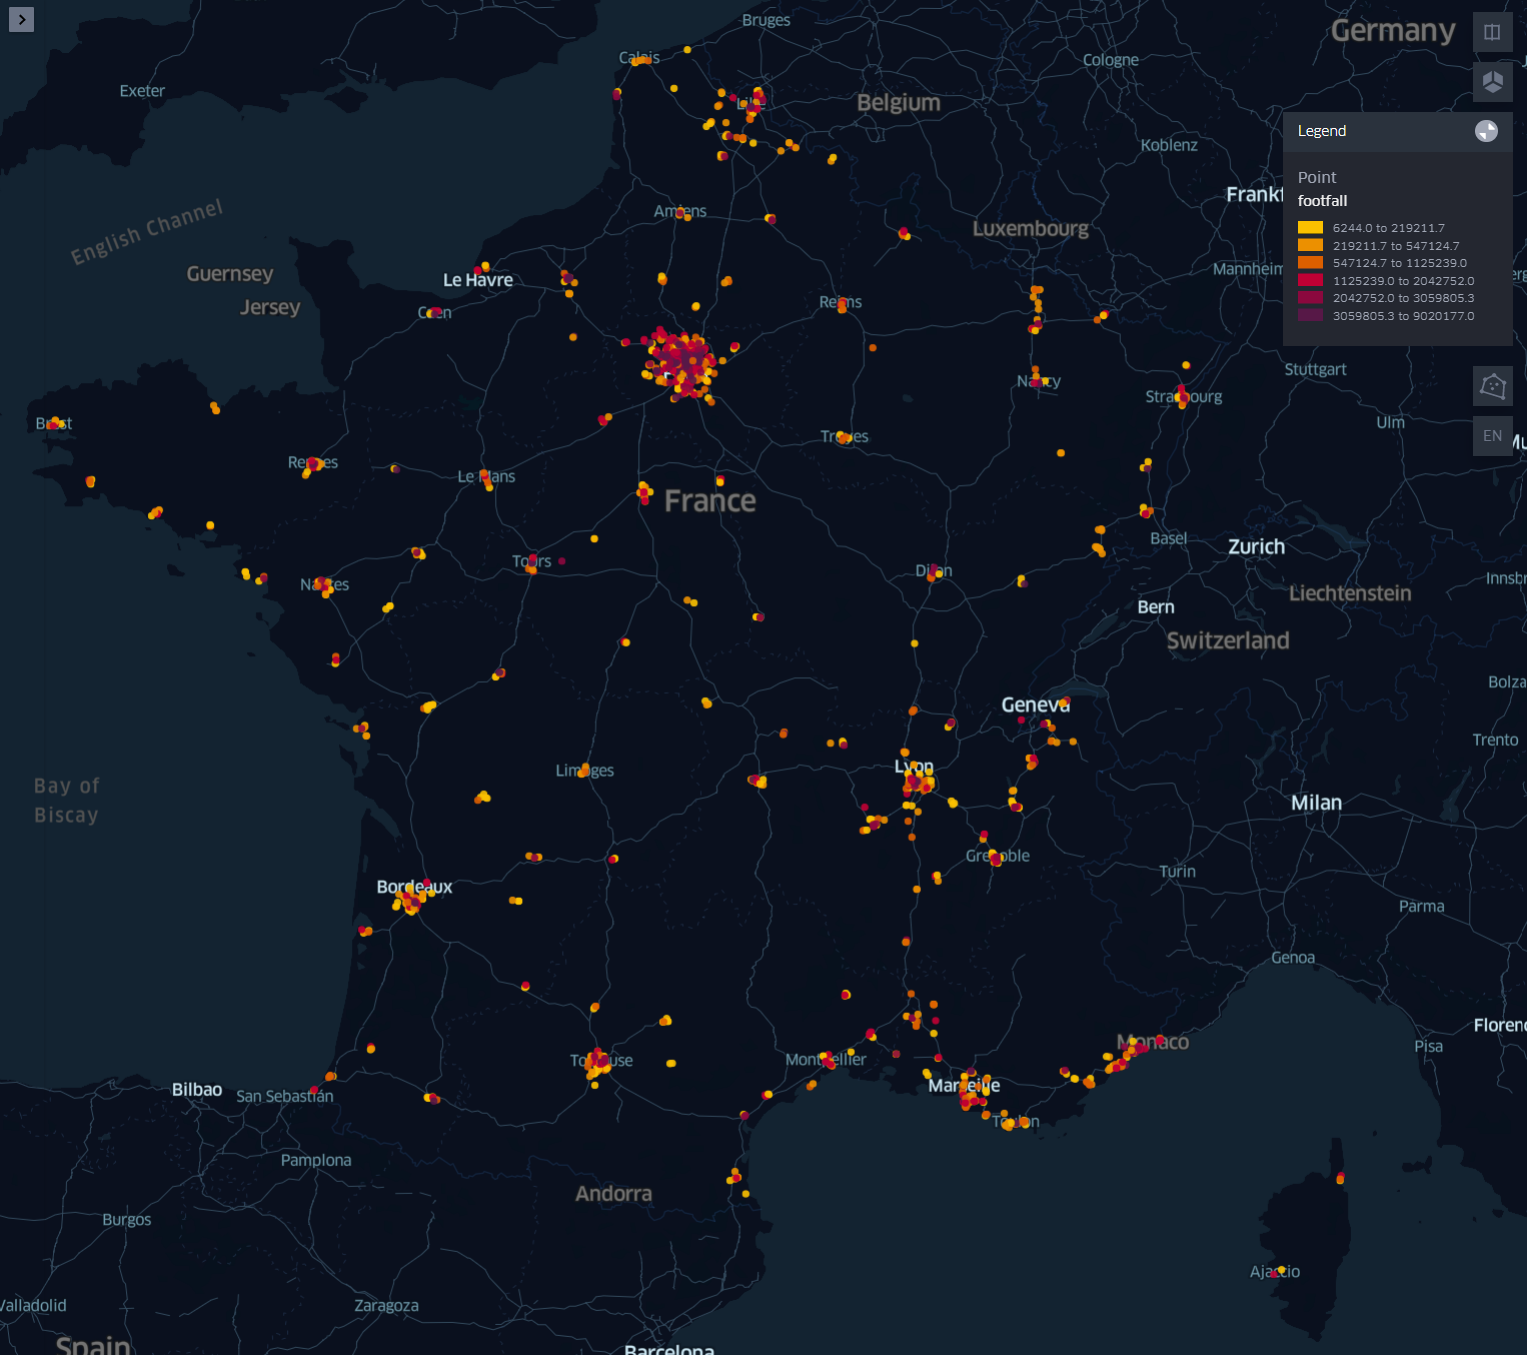
\includegraphics[width=\linewidth]{images/graphs/map_of_label_footfall.png}
    \caption{Carte des données d'entraînement}
    \label{fig:footfallmap}
\end{figure}

\subsection{Technologies utilisées}

\subsubsection{Agrégation spatiale}

Une fois que nous avons l'ensemble de nos données on remarque qu'elles se distingue en deux groupes de par leur nature. Les données ponctuelles (\'Evènements de visites, POI, etc.) et les données surfaciques (Population par IRIS). Pour homogénéiser notre donnée et simplifier les futurs calculs il est important de segmenter l'espaces et ajouter un index spatial à nos données.

Nous nous sommes dirigé vers la solution des hexagones H3 \cite{Uber_H3} développé par Uber. C'est un système d'indexation géospatiale qui constitue un pavage hexagonal de la sphère multi-échelles et dont les index sont hiérarchiques.

Dans notre cas c'est la solution optimale car nous pouvons l'utiliser pour joindre nos données disparates, le format hexagonal facilite la modélisation des flux et est bien adapté pour appliquer le machine learning aux données géospatiales.


% Image of the offices
\begin{figure}[H]
    \centering
    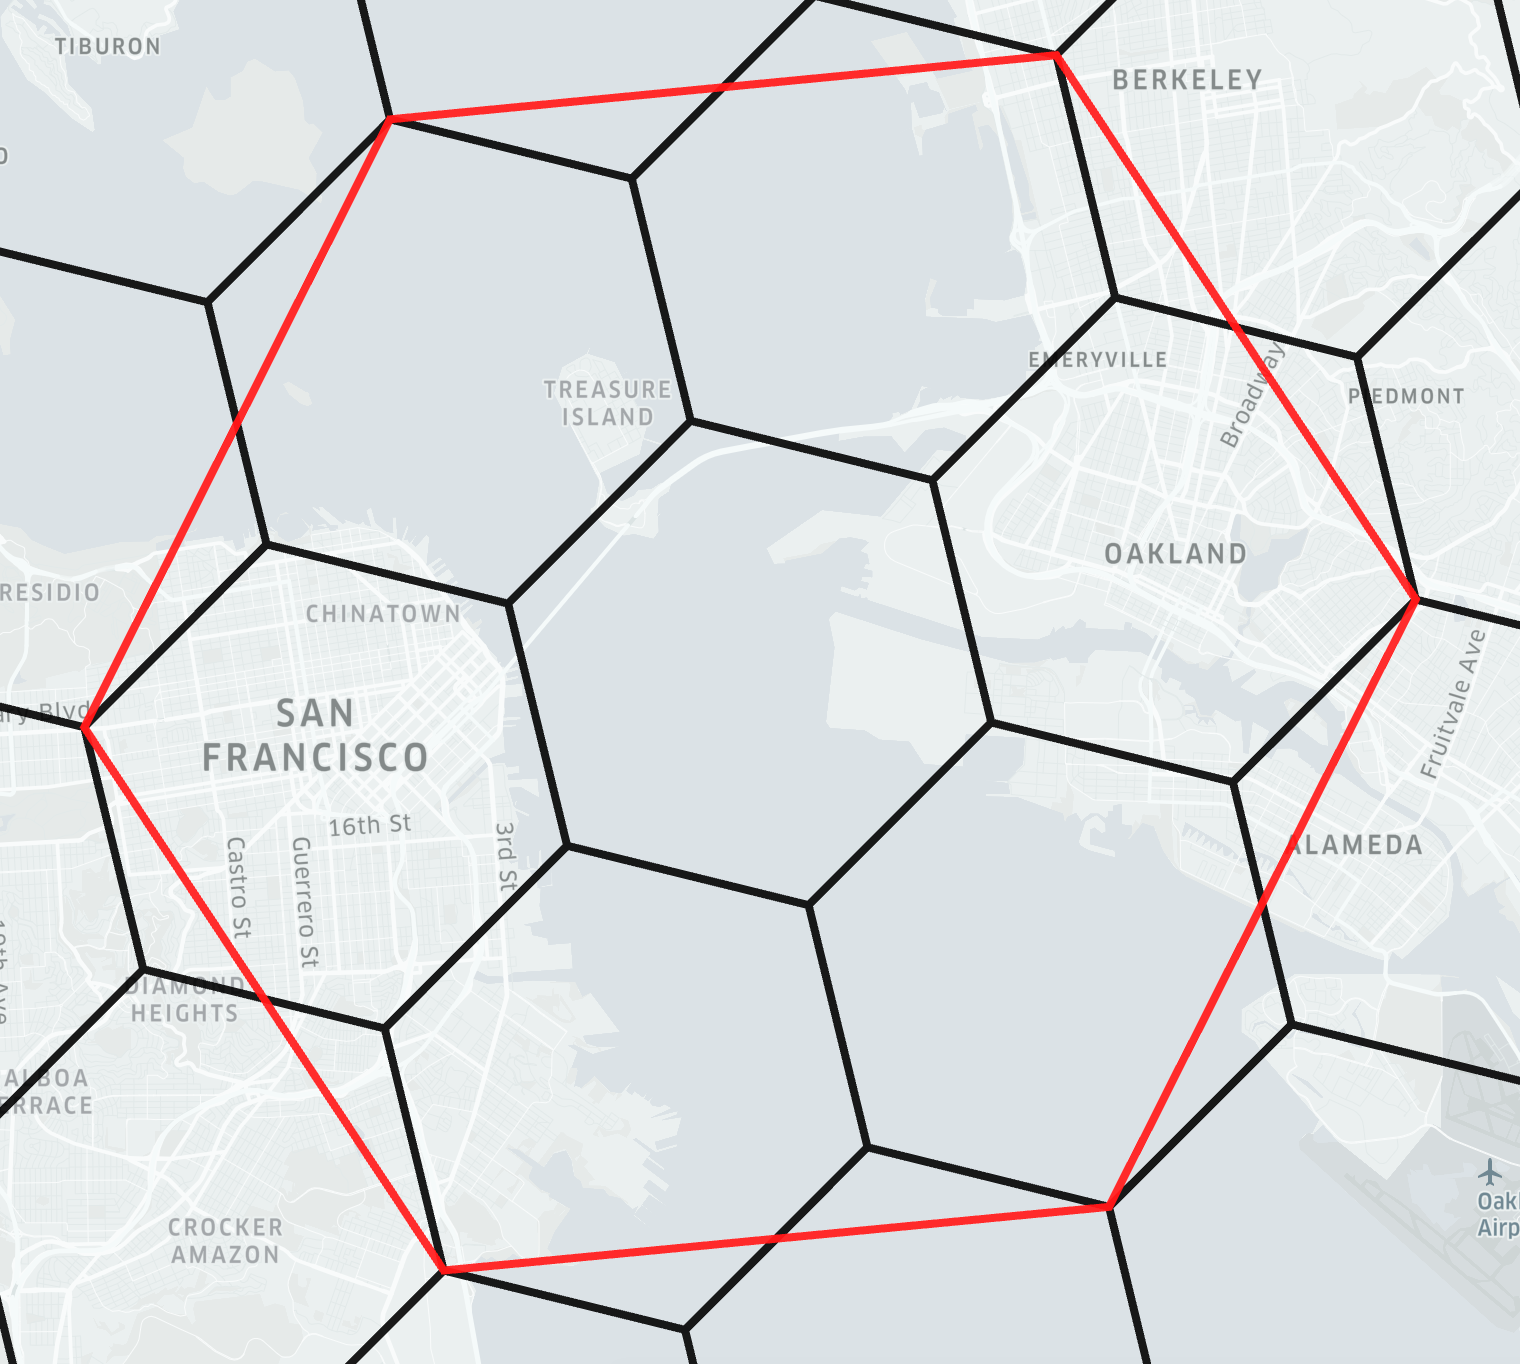
\includegraphics[width=7cm]{images/graphs/h3-multiscale.png}
    \caption{Principe de multi-echelles des cellules H3}
    \label{fig:celluleh3}
\end{figure}

\begin{figure}[H]
    \centering
    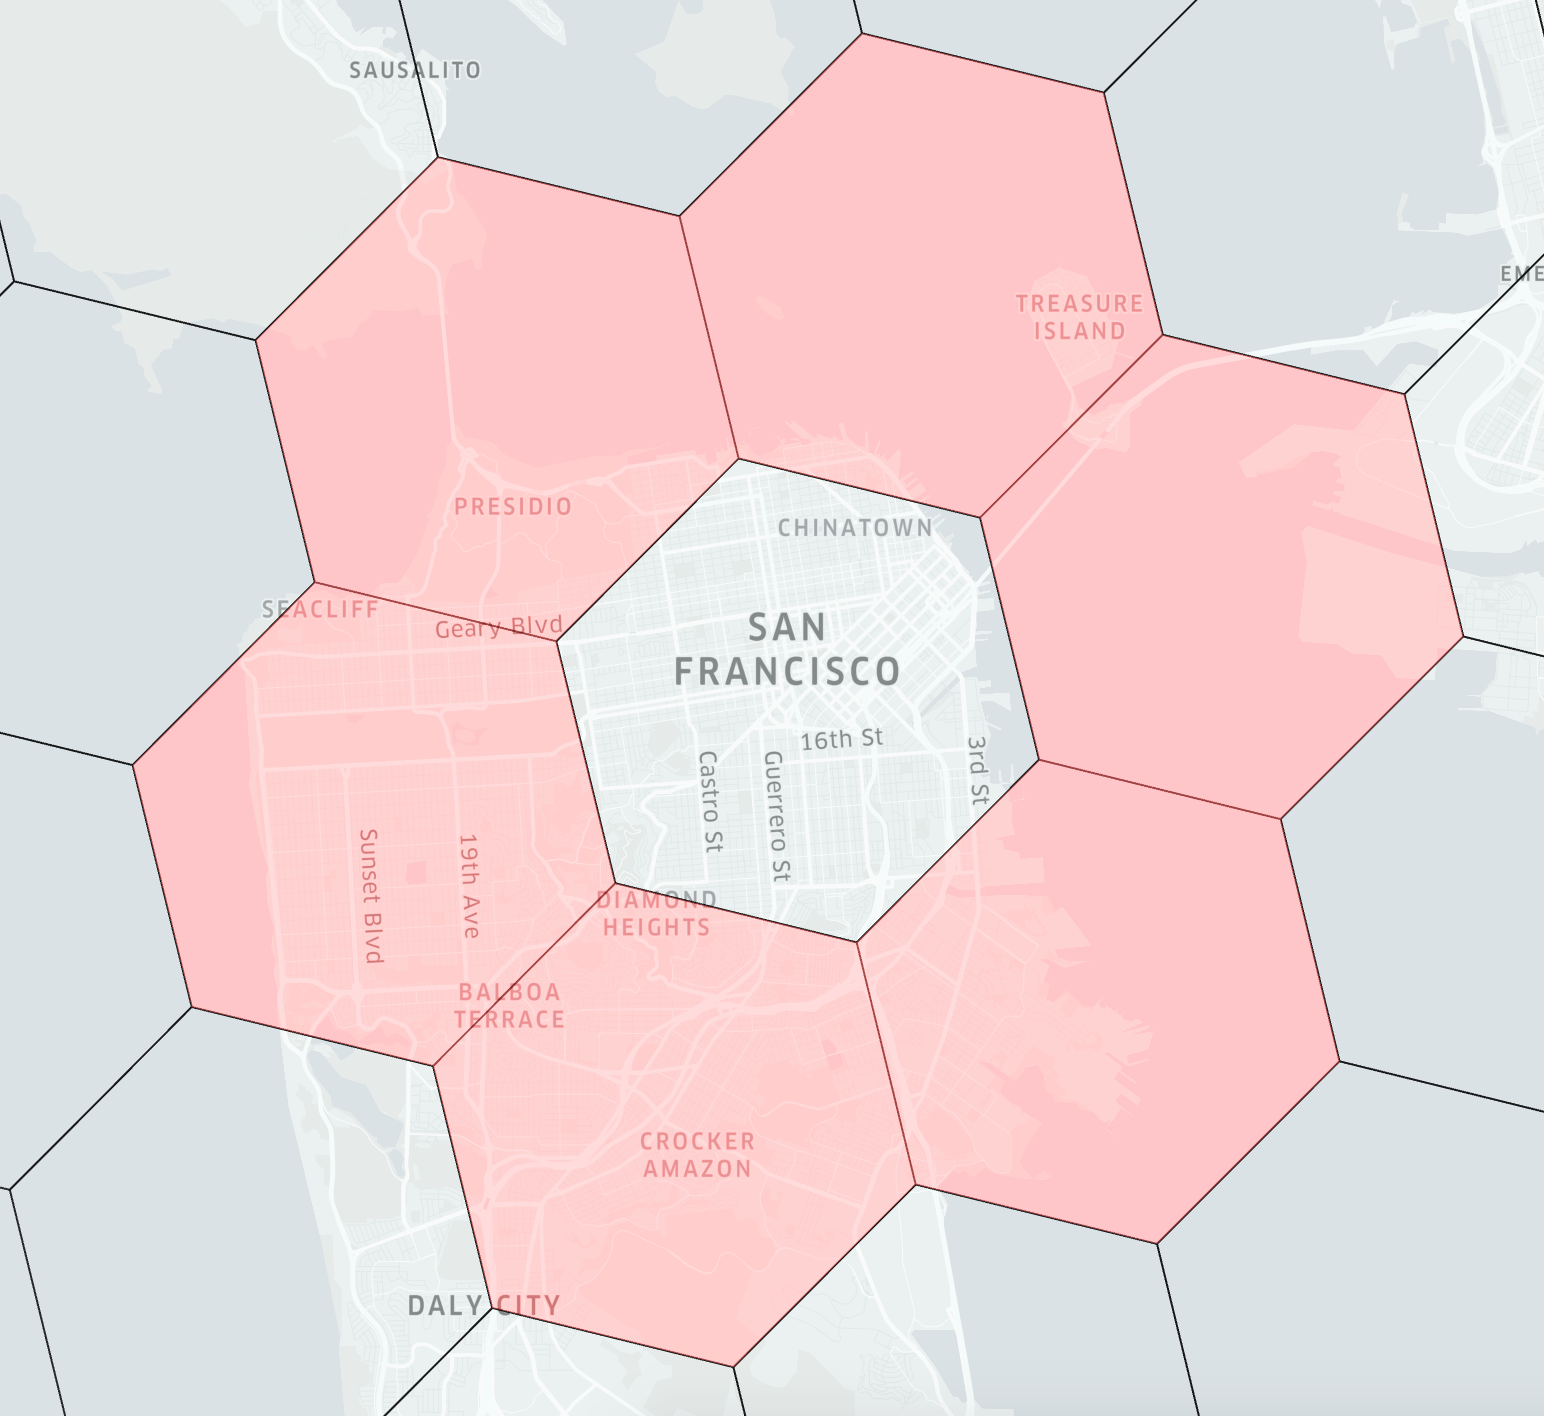
\includegraphics[width=7cm]{images/graphs/h3-ring.png}
    \captionsetup{justification=centering}
    \caption{Les 6 voisins d'une cellule H3 se rapproche d'un cercle, utile pour la modélisation de flux}
    \label{fig:celluleh3ring}
\end{figure}

Pour notre part on choisira le niveau d'échelle 11, ce qui correspond environ à un hexagone de 27 mètres de rayon.

\subsubsection{Infrasture de base de donnée}

Pour stocker toutes ces données, Galigeo utilise un service de Cloud Computing \footnote{A compléter} nommé Google Cloud Plateform (GCP) qui permet de stocker une grande quantité de donnée et de faire des calculs plus ou moins complexe sur celle-ci.

\paragraph*{}

Un des grands avantages de cette solution est l'intégration de Tensorflow, une bibliothèque open-source développé par Google pour faire du machine learning et de l'intelligence artificielle. Elle est très utile pour l'entraînement de réseaux de neurones profonds (DNN).

Nous pouvons également y combiner Keras, une interface open-source conçu pour simplifier l'utilisation de Tensorflow.


\subsubsection{Type de modèle utilisé}

\'Etant donné les choix précédents, nous nous sommes donc orientés vers un modèle de Deep Neural Network (DNN).

Il est cependant important de noté que les modèles de Deep Neural Network, prouve leur meilleure efficacité par rapport à d'autre modèle de Machine Learning lorsque la donnée est non structurée et que la taille du dataset \footnote{A compléter} est importantes (plusieurs millions de lignes)

Dans notre cas, ces conditions ne sont pas remplies mais nous verrons plus tard dans ce rapport les alternatives envisagées.


\subsection{Préparation des données}

\subsubsection{Structuration des données}

Cette étape est cruciale pour obtenir des bons résultats après la modélisation. Il s'agit de passer de la donnée brute présentée précédemment à une donnée structurée qui permettra d'entraîner le réseau de neurones.

Pour cela, nous avons projeté l'ensemble de notre donnée brute sur la grille H3 d'Uber. Pour chaque valeur de flux piéton mesuré, nous avons calculé le nombre de visites dans la même cellule ainsi que dans les cellules voisines. Nous avons agrégé ces données events par mois sur une année complète de septembre 2021 à août 2022.

Nous avons appliqué le même principe spatial pour les POIs. Les cellules voisines se calcul très facilement grâce aux fonctions open-source mise à disposition. Ainsi on peut calculer différents anneaux autour de notre cellule de départ.


\begin{figure}[H]
    \centering
    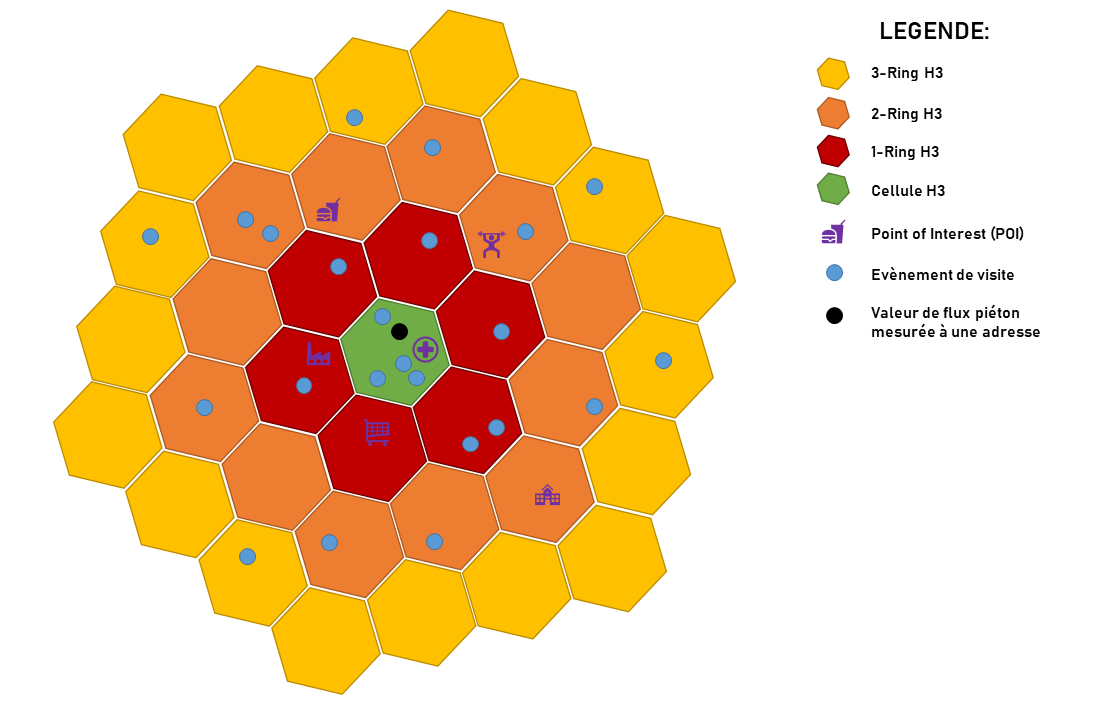
\includegraphics[width=\linewidth]{images/graphs/dataset.png}
    \captionsetup{justification=centering}
    \caption{Agrégation des données aux cellules H3 pour générer un dataset}
    \label{fig:dataset_aggregation}
\end{figure}

Pour ce qui est de la donnée de population, nous avons simplement pris le centroïde de la cellule H3, et l'avons intersecté avec les géométries des IRIS françaises afin de déterminé dans quel IRIS la cellule se trouve.

Nous avons obtenu alors une structure de dataset comme ci-dessous. Une feature est un paramètre du modèle et le label est la variable à estimer.


\begin{table}[H]
    \centering
    \begin{tabular}{|l|l|l|}
    \hline
    \textbf{Colonnes}    & \textbf{Type} & \textbf{Description}                                                    \\ \hline
    h3\_index            &               & Index de la cellule H3                                                  \\ \hline
    visits\_MMAAAA & feature       & Nb events dans la cellule H3 par mois (x12)                        \\ \hline
    visits        & feature       & Nb events dans la cellule H3 sur l'année                          \\ \hline
    visits\_k1     & feature       & Nb events dans la cellule H3 et l'anneau 1 sur l'année            \\ \hline
    visits\_k2     & feature       & Nb events dans la cellule H3 et les annaux 1, 2 sur l'année       \\ \hline
    visits\_k3     & feature       & Nb events dans la cellule H3 et les annaux 1, 2, 3 sur l'année    \\ \hline
    visits\_k4     & feature       & Nb events dans la cellule H3 et les annaux 1, 2, 3, 4 sur l'année \\ \hline
    poi\_N        & feature       & Nb de POI dans la cellule H3 par nature                                 \\ \hline
    poi\_N\_k1    & feature       & Nb de POI dans la cellule H3 et l'anneau 1 par nature                   \\ \hline
    poi\_N\_k2    & feature       & Nb de POI dans la cellule H3 et les annaux 1, 2 par nature              \\ \hline
    poi\_N\_k3    & feature       & Nb de POI dans la cellule H3 et les annaux 1, 2, 3 par nature           \\ \hline
    poi\_N\_k4    & feature       & Nb de POI dans la cellule H3 et les annaux 1, 2 , 3 , 4 par nature      \\ \hline
    population           & feature       & Population in the IRIS of the H3 cell                                   \\ \hline
    footfall             & label         & Flux piéton mesuré en un point de la cellule H3                         \\ \hline
    \end{tabular}
    \caption{Structure du dataset}
    \end{table}

On obtient alors un dataset d'environ 11000 lignes et 14 colonnes.

\subsubsection{Nettoyage des données}

La deuxième étape de la préparation des données consiste à les nettoyer pour supprimer d'abords les lignes où il manquerait certaines variables puis celle dont les valeurs du label sont aberrantes.

On se retrouve alors avec un dataset réduit de 40\%, il reste environ 6500 lignes.

\paragraph{}


Une fois ces deux étapes réalisées, nous pouvons sortir différents graphiques statistiques disponible en annexe : KDE, Matrice de corrélation, Répartitions des features.


\subsection{Tuner et Entraînement du modèle}

Notre dataset est maintenant prêt à être utilisé comme base d'apprentissage. Nous avons donc créé une structure de modèle. Cette structure possède des paramètres appelés Hyperparamètres. Chaque hyperparamètre peut prendre une valeur parmi une liste bien définie. Le principe du Tuner est de compiler ce modèle plusieurs fois avec des valeurs d'hyperparamètre bien différentes et choisies aléatoirement.

\begin{figure}[H]
    \centering
    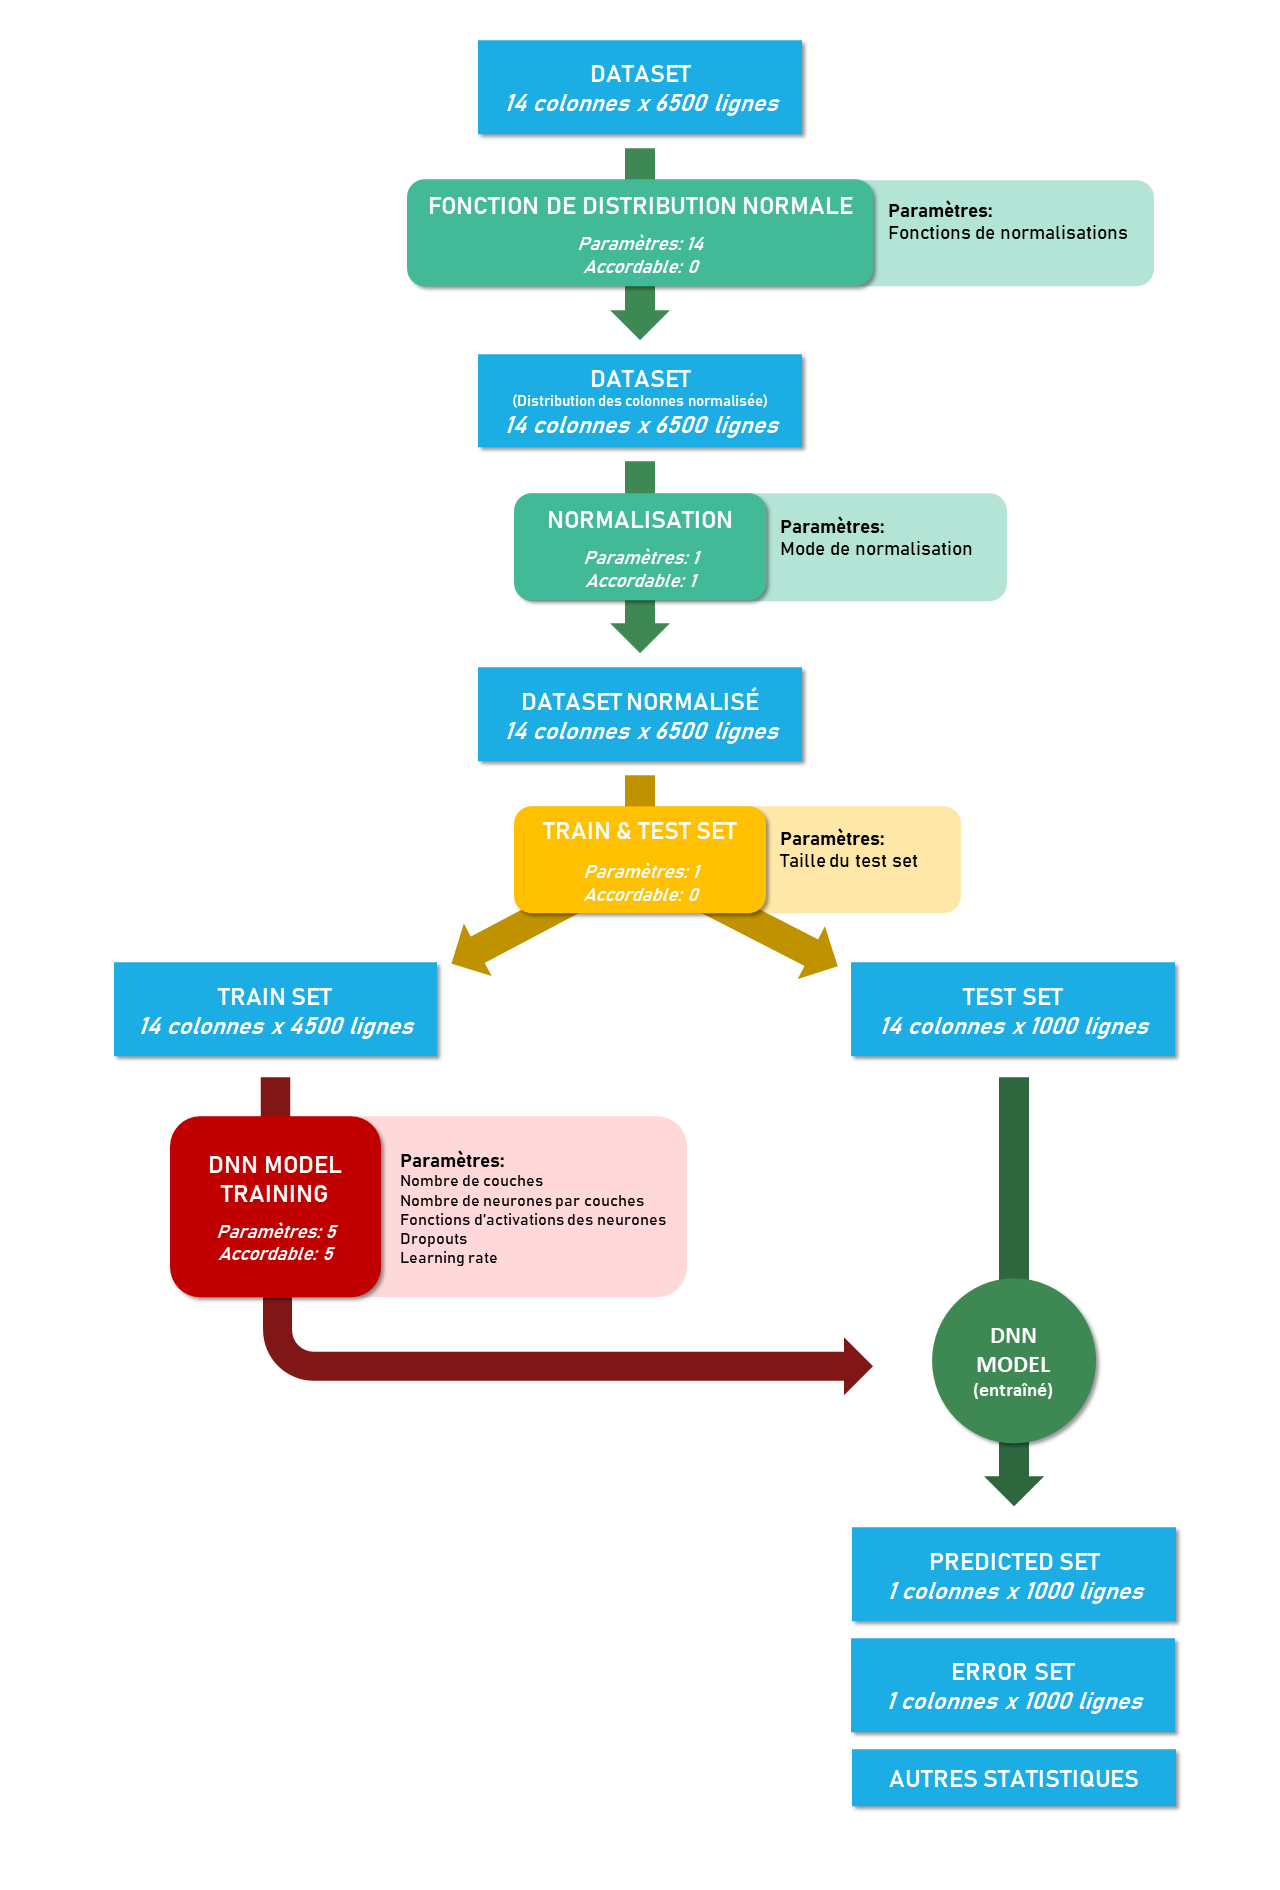
\includegraphics[width=\linewidth]{images/graphs/struc_model_dnn.png}
    \captionsetup{justification=centering}
    \caption{Structure du modèle envisagé}
    \label{fig:strcu_dnn}
\end{figure}

La première étape de notre modèle est donc de normaliser la distribution de nos features. En effet, la distribution des valeurs pour chaque features n'est pas forcément "normale" et il est préférable de passer nos valeurs à travers une fonction pour la modifier.

\begin{figure}[H]
    \centering
    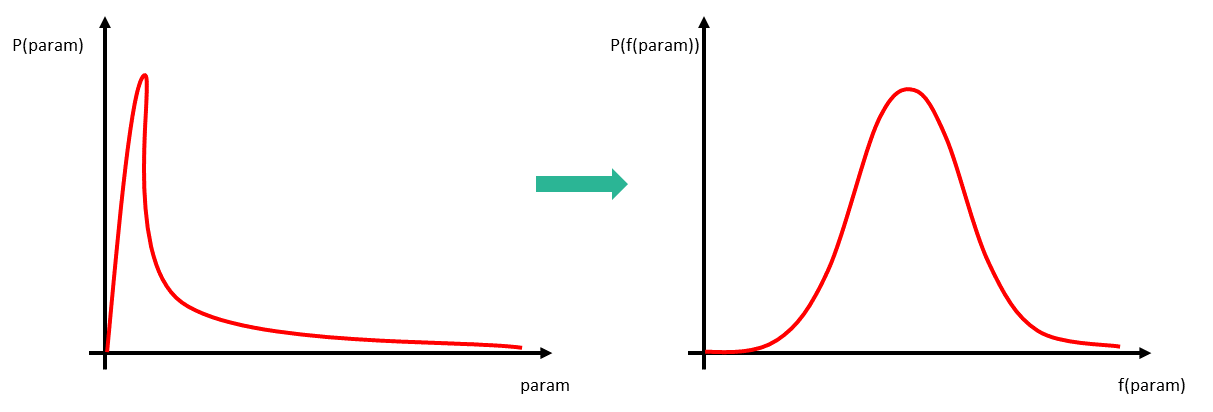
\includegraphics[width=\linewidth]{images/graphs/fct_histo.png}
    \captionsetup{justification=centering}
    \caption{Principe de normalisation de la distribution d'une feature}
    \label{fig:fct_repartition}
\end{figure}

L'étape suivante est de normaliser les valeurs de nos features (cette fois ci, on ne modifie pas le label). Pour cela, il existe principalement deux types de normalisation : La normalisation min/max et la normalisation moyenne/écart-type.

Cela permet entre autres d'assurer une cohérence entre les données et permet à l'exécution d'être plus rapide et meilleure.


\paragraph{}

Une fois cette étape réalisée, nous divisons en deux partie aléatoire (la proportion est contrôlée) le dataset normalisé. La partie "trainset" permet d'entraîner le modèle et la partie "testset" permet de vérifier si le modèle est correctement entraîné.

\paragraph{}

L'objectif est maintenant d'obtenir un réseau de neurones entraîné. Pour cela, nous utilisons un modèle construit sur les hyperparamètres et lui passons l'ensemble du trainset en entré. En parcourant l'ensemble des données et en essayant d'estimer le label, le réseau de neurone apprend et règle ses paramètres internes (poids des axones, valeur interne des neurones, etc.) en appliquant une validation croisée.

De cette étape, nous récupérons un réseau de neurones profonds qui permet maintenant d'estimer notre label en fonction de nos features.


\paragraph{}

Nous passons donc notre testset dans notre réseau neuronal. Cela nous permet d'obtenir notre label estimé et de le comparer au vrai label. On obtient alors une liste de n erreurs (dans notre cas 1000), grâce auxquels nous pouvons mesurer la qualité du réseau de neurones. On peut calculer l'erreur quadratique moyenne (RMSE), un coefficient de détermination (R2) ou la précision du modèle ("accuracy").

\subsection{Résultats}

A COMPLETER

\section{Prédiction de chiffre d'affaire}

\subsection{Contexte}

Une des manière pour qu'une entreprise continue à croître

\subsection{Données}

\subsection{Structure du modèle}

\subsection{Résultats}

\section{Autres missions}

\subsection{Analyse de données - Base de donnée nationale des Bâtiments}

\subsection{Data engineering - Scrapping et automatisation de chaîne d'acquisition de données}